\documentclass[a4paper,12pt]{article}
\usepackage{graphicx}
\usepackage{circuitikz}
\usepackage{amsmath}
\usepackage{booktabs}
\usepackage{hyperref}
\usepackage{caption}
\usepackage{float}
\title{\textbf{Design and Implementation of a Mod-7 Asynchronous Counter}}
\author{EE24BTECH11021-ESHAN RAY\\ EE24BTECH11048-NITHIN.K}


\begin{document}

\maketitle

\begin{abstract}
This lab report presents the design, implementation, and testing of a Mod-7 asynchronous counter using JK flip-flops. The counter operates with an external clock signal provided by an Arduino and its performance is verified using a Cathode Ray Oscilloscope (CRO).
\end{abstract}

\section{Introduction}
A Mod-7 counter is a sequential circuit that counts from 0 to 6 and then resets to 0. Using JK flip-flops in a toggle mode, the counter progresses through seven states. The asynchronous nature means that each flip-flop's clock input is triggered by the output of the previous flip-flop.

\section{Components and Equipment}
\begin{itemize}
    \item JK Flip-Flops (e.g., 7476 IC)
    \item NAND gate(e.g. , 7410 IC)
    \item Arduino (as a clock source)
    \item 3 LED's
    \item Cathode Ray Oscilloscope (CRO)
    \item Resistors and Capacitors (as needed)
    \item Connecting Wires and Breadboard
    \item Power Supply (5V DC)
\end{itemize}

\section{Circuit Design}
The Mod-7 counter is implemented using three JK flip-flops. The JK flip-flops are configured in toggle mode by connecting both J and K inputs to logic HIGH (1). The clock for the first flip-flop is provided by the Arduino, while subsequent flip-flops receive their clock signal from the previous flip-flop's output.

\subsection{Conversion of JK Flip-Flop to T Flip-Flop}
A JK Flip-Flop can be converted into a T Flip-Flop by making the following modifications:
\begin{table}[H]
    \centering
    \begin{tabular}{|c|c|c|}
        \hline
        \textbf{T} & \textbf{Q (Previous State)} & \textbf{Q (Next State)} \\
        \hline
        0 & 0 & 0 \\
        0 & 1 & 1 \\
        1 & 0 & 1 \\
        1 & 1 & 0 \\
        \hline
    \end{tabular}
    \caption{Truth Table for T Flip-Flop}
\end{table}
\begin{table}[H]
    \centering
    \begin{tabular}{|c|c|c|c|}
        \hline
        \textbf{J} & \textbf{K} & \textbf{Q (Previous State)} & \textbf{Q (Next State)} \\
        \hline
        0 & 0 & 0 & 0 \\
        0 & 0 & 1 & 1 \\
        0 & 1 & 0 & 0 \\
        0 & 1 & 1 & 0 \\
        1 & 0 & 0 & 1 \\
        1 & 0 & 1 & 1 \\
        1 & 1 & 0 & 1 \\
        1 & 1 & 1 & 0 \\
        \hline
    \end{tabular}
    \caption{Truth Table for JK Flip-Flop}
\end{table}
\begin{table}[H]
    \centering
    \begin{tabular}{|c|c|c|c|c|}
        \hline
        \textbf{Q} & \textbf{T} & \textbf{J} & \textbf{K} & \textbf{Q ( Next State)} \\
        \hline
        0 & 0 & 0 & X & 0 \\
        0 & 1 & 1 & X & 1 \\
        1 & 0 & X & 0 & 1 \\
        1 & 1 & X & 1 & 0 \\
        \hline
    \end{tabular}
    \caption{Truth Table for JK to T Flip-Flop}
\end{table}

\begin{enumerate}
    \item Connect both J and K inputs together.
    \item Use a single toggle (T) input instead of separate J and K inputs.
    \item The T input determines the flip-flop's behavior:
          \begin{itemize}
              \item When \( T = 0 \), the output remains unchanged.
              \item When \( T = 1 \), the output toggles.
          \end{itemize}
\end{enumerate}
Since the Mod-7 counter requires toggle functionality, we connect J = K = 1 for each flip-flop, effectively making them act as T Flip-Flops.

\subsection{State Transition Table}
\begin{table}[H]
    \centering
    \begin{tabular}{c c c | c c c}
        \toprule
        \multicolumn{3}{c|}{Current State} & \multicolumn{3}{c}{Next State} \\
        Q3 & Q2 & Q1 & Q3 & Q2 & Q1 \\
        \midrule
        0 & 0 & 0 & 0 & 0 & 1 \\
        0 & 0 & 1 & 0 & 1 & 0 \\
        0 & 1 & 0 & 0 & 1 & 1 \\
        0 & 1 & 1 & 1 & 0 & 0 \\
        1 & 0 & 0 & 1 & 0 & 1 \\
        1 & 0 & 1 & 1 & 1 & 0 \\
        1 & 1 & 0 & 0 & 0 & 0 \\
        \bottomrule
    \end{tabular}
    \caption{State Transition Table for Mod-7 Counter}
\end{table}
\newpage
\subsection{Circuit Diagram}
\begin{figure}[H]
\centering
       \begin{circuitikz}[scale=0.85]
\tikzstyle{every node}=[font=\normalsize]
\draw  (6.25,10) rectangle (7.75,8.25);
\draw  (9.5,10) rectangle (11,8.25);
\draw  (12.5,10) rectangle (13.75,8.25);
\draw [short] (4,9.75) -- (6.25,9.75);
\draw [short] (4.25,8.5) -- (6.25,8.5);
\draw [short] (4,9) -- (6.25,9);
\draw [short] (7.75,9) -- (9.5,9);
\draw [short] (5.25,9.75) -- (5.25,11.25);
\draw [short] (5.25,11.25) -- (8,11.25);
\draw [short] (8,11.25) -- (8,9.75);
\draw [short] (8,9.75) -- (9.5,9.75);
\draw [short] (5.25,8.5) -- (5.25,7.5);
\draw [short] (5.25,7.5) -- (8.5,7.5);
\draw [short] (8.5,7.5) -- (8.5,8.5);
\draw [short] (8.5,8.5) -- (9.5,8.5);
\draw [short] (11,9) -- (12.5,9);
\draw [short] (8.75,9.75) -- (8.75,10.75);
\draw [short] (8.75,10.75) -- (11.5,10.75);
\draw [short] (11.5,10.75) -- (11.5,9.75);
\draw [short] (11.5,9.75) -- (12.5,9.75);
\draw [short] (8.75,8.5) -- (8.75,7.5);
\draw [short] (8.75,7.5) -- (11.75,7.5);
\draw [short] (11.75,7.5) -- (11.75,8.5);
\draw [short] (11.75,8.5) -- (12.5,8.5);
\draw [short] (13.75,9) -- (14.75,9);
\draw (16.5,6.75) to[short] (16.75,6.75);
\draw (16.5,6.25) to[short] (16.75,6.25);
\draw (16.75,6.75) node[ieeestd nand port, anchor=in 1, scale=0.89](port){} (port.out) to[short] (18.5,6.5);
\draw (14.75,9) to[short] (14.75,6.75);
\draw (14.75,6.75) to[short] (16.5,6.75);
\draw (17.2,6.5) to[short] (11.5,6.5);
\draw (11.5,6.5) to[short] (11.5,9);
\draw (16.75,6.2) to[short] (8.25,6.2);
\draw (8.25,6.2) to[short] (8.25,9);
\draw (18.9,6.45) to[short] (19.5,6.45);
\draw (19.5,6.45) to[short] (19.5,4.5);
\draw (7,8.25) to[short, -o] (7,7.75) ;
\draw (19.5,4.5) to[short] (7,4.5);
\draw (7,4.5) to[short] (7,7.75);
\draw (10.25,8.25) to[short, -o] (10.25,7.75) ;
\draw (13.25,8.25) to[short, -o] (13.25,7.75) ;
\draw (7,7.75) to[short] (13.25,7.75);
\draw  (6.5,13.75) rectangle (13.25,12.75);
\node [font=\Large] at (9.75,13.25) {Power Supply};
\draw (7,10) to[short, -o] (7,10.5) ;
\draw (10.25,10) to[short, -o] (10.25,10.5) ;
\draw (13,10) to[short, -o] (13,10.5) ;
\draw (13,10.5) to[short] (13,12.75);
\draw (10.25,10.5) to[short] (10.25,12.75);
\draw (7,10.5) to[short] (7,12.75);
\draw  (0,13.75) rectangle (4,12.75);
\node [font=\Large] at (2,13.25) {Normal Clock};
\draw [short] (4,9) -- (2,9);
\draw [short] (2,9) -- (0.25,9);
\draw [short] (0.25,9) -- (0.25,12.75);
\draw [short] (4.5,8.5) -- (3,8.5);
\draw [short] (3,8.5) -- (3,11.75);
\draw [short] (3,11.75) -- (4.5,11.75);
\draw [short] (4.5,11.75) -- (4.5,13.25);
\draw [short] (4.5,13.25) -- (6.5,13.25);
\draw [short] (4,9.75) -- (3.75,9.75);
\draw [short] (3.75,9.75) -- (3.75,11.75);
\node [font=\large] at (7,9.15) {JK};
\node [font=\large] at (10.25,9.15) {JK};
\node [font=\large] at (13.15,9.15) {JK};
\node [font=\large] at (8.2,9.25) {Q1};
\node [font=\large] at (11.4,9.25) {Q2};
\node [font=\large] at (14.2,9.25) {Q3};
\node [font=\small] at (7,9.75) {PRT};
\node [font=\small] at (10.25,9.75) {PRT};
\node [font=\small] at (13.1,9.75) {PRT};
\node [font=\small] at (7,8.5) {CLR};
\node [font=\small] at (10.25,8.5) {CLR};
\node [font=\small] at (13.2,8.5) {CLR};
\node [font=\large] at (6,9.75) {J};
\node [font=\large] at (9.25,9.75) {J};
\node [font=\large] at (12.25,9.75) {J};
\node [font=\large] at (6,8.5) {K};
\node [font=\large] at (9.25,8.5) {K};
\node [font=\large] at (12.25,8.5) {K};
\end{circuitikz}
\caption*{Circuit Diagram for Mod-7 Counter using JK Flip-Flops}
\end{figure}

\section{Implementation}
The Arduino generates a clock signal using the following code:

\begin{verbatim}
#define CLOCK_PIN 8
void setup() {
    pinMode(CLOCK_PIN, OUTPUT);
}

void loop() {
    digitalWrite(CLOCK_PIN, HIGH);
    delay(100);
    digitalWrite(CLOCK_PIN, LOW);
    delay(100);
}
\end{verbatim}

\section{Procedure}

\begin{enumerate}
    \item \textbf{Circuit Assembly}
    \begin{enumerate}
        \item Connect three JK flip-flops in cascade to form the Mod-7 counter.
        \item Configure each JK flip-flop in toggle mode by connecting \( J = 1 \) and \( K = 1 \).
        \item Use a NAND gate to reset the counter when the state reaches 7 (111).
        \item Connect LEDs to the output of each flip-flop to visualize the counting sequence.
        \item Provide power (5V) and ground connections to all ICs.
    \end{enumerate}

    \item \textbf{Clock Signal Generation}
    \begin{enumerate}
        \item Use an Arduino to generate a square wave clock signal at a fixed frequency.
        \item Connect the Arduino clock output to the clock input of the first flip-flop.
        \item Verify the clock signal using an oscilloscope.
    \end{enumerate}

    \item \textbf{Counter Operation Testing}
    \begin{enumerate}
        \item Power the circuit and observe the LED sequence.
        \item Verify the counting sequence from 000 to 110 and check that it resets to 000.
        \item Use a CRO to capture and analyze the waveforms of the clock and output states.
        \item Measure the frequency division to confirm \( f_{Q1} = \frac{f_{clk}}{2} \), \( f_{Q2} = \frac{f_{clk}}{4} \), and \( f_{Q3} = \frac{f_{clk}}{8} \).
    \end{enumerate}

    \item \textbf{Analysis and Verification}
    \begin{enumerate}
        \item Compare the observed outputs with the theoretical state transition table.
        \item Ensure proper synchronization of flip-flops and confirm correct reset behavior.
    \end{enumerate}
\end{enumerate}

\section{Observations and Results}
The counter output was verified using a Cathode Ray Oscilloscope (CRO), showing the expected sequence from 000 to 110 before resetting. The waveform analysis confirmed the correct operation of the Mod-7 counter.
The below pictures are of the LED counter:\\
\textbf{The LED blinking represents 1 and the order is Q3, Q2, Q1 from left to right:}
\begin{figure}[H]
\centering
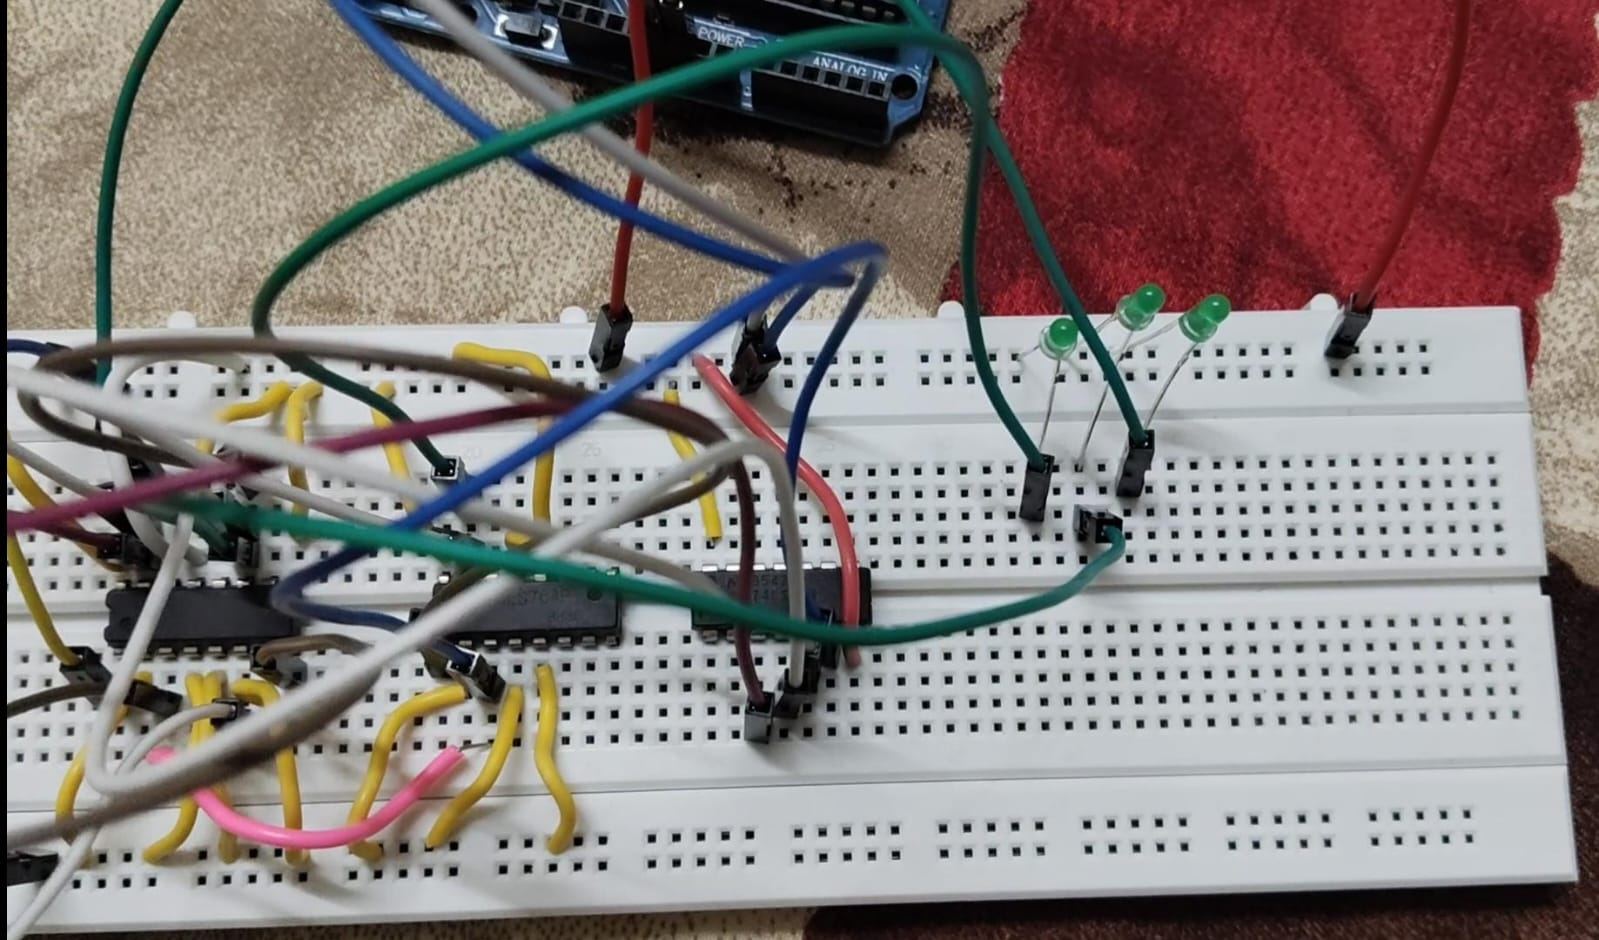
\includegraphics[width=0.6\textwidth]{figs/1.jpeg}
\caption*{0 0 0 = 0}
\end{figure}
\begin{figure}[H]
\centering
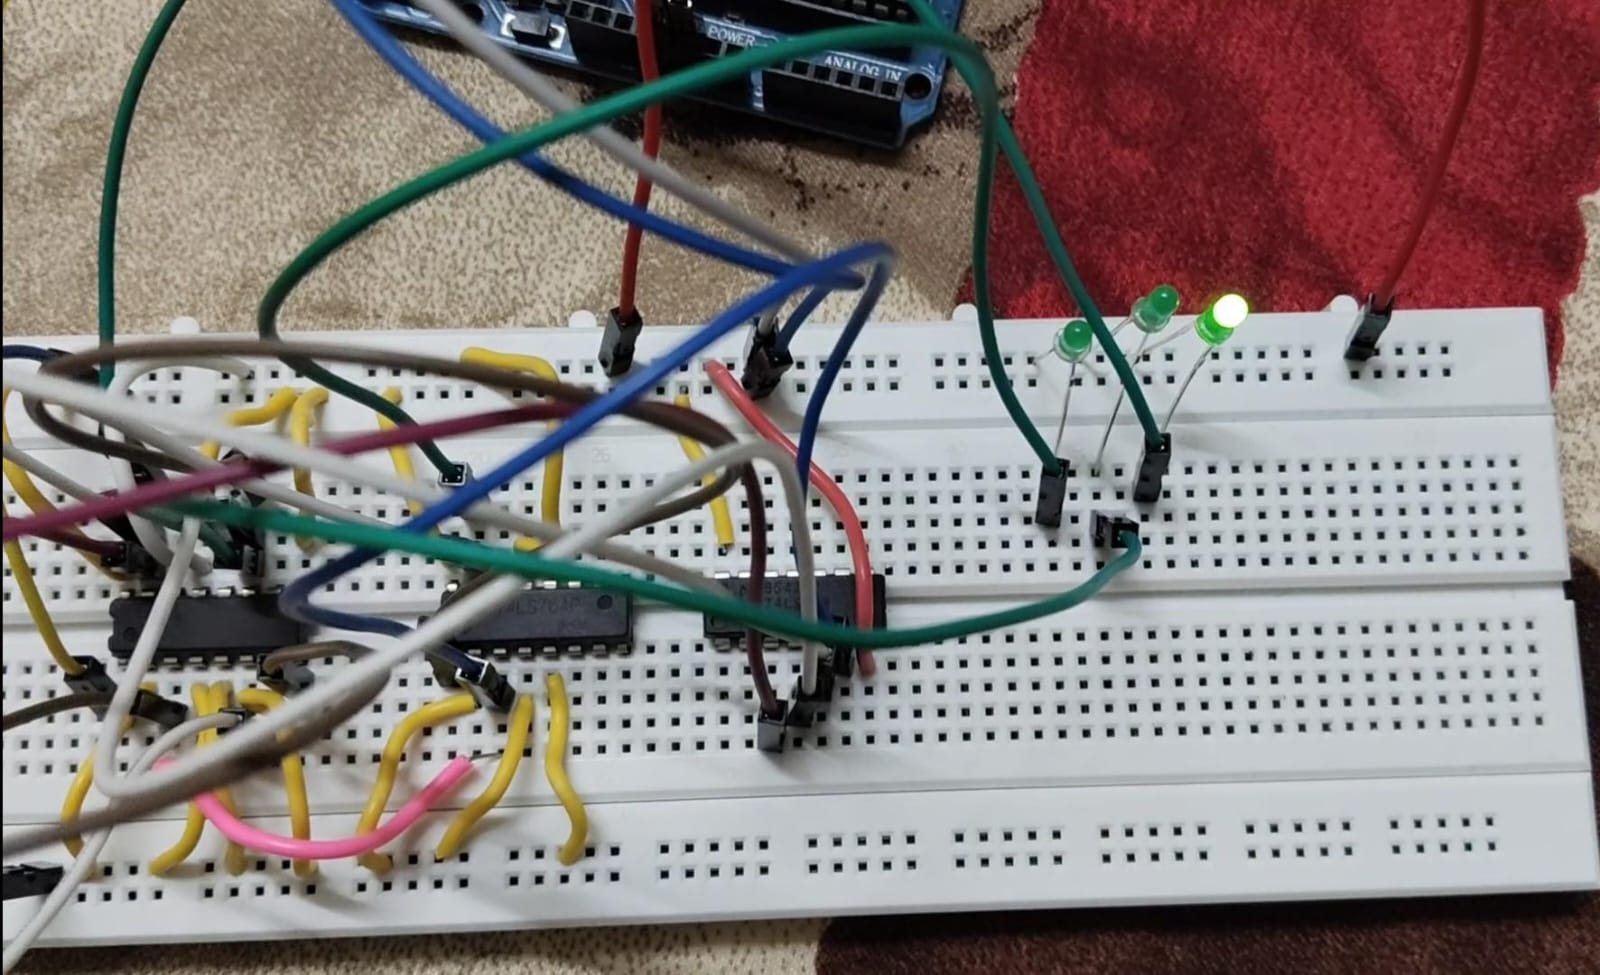
\includegraphics[width=0.6\textwidth]{figs/2.jpeg}
\caption*{0 0 1 = 1}
\end{figure}
\begin{figure}[H]
\centering
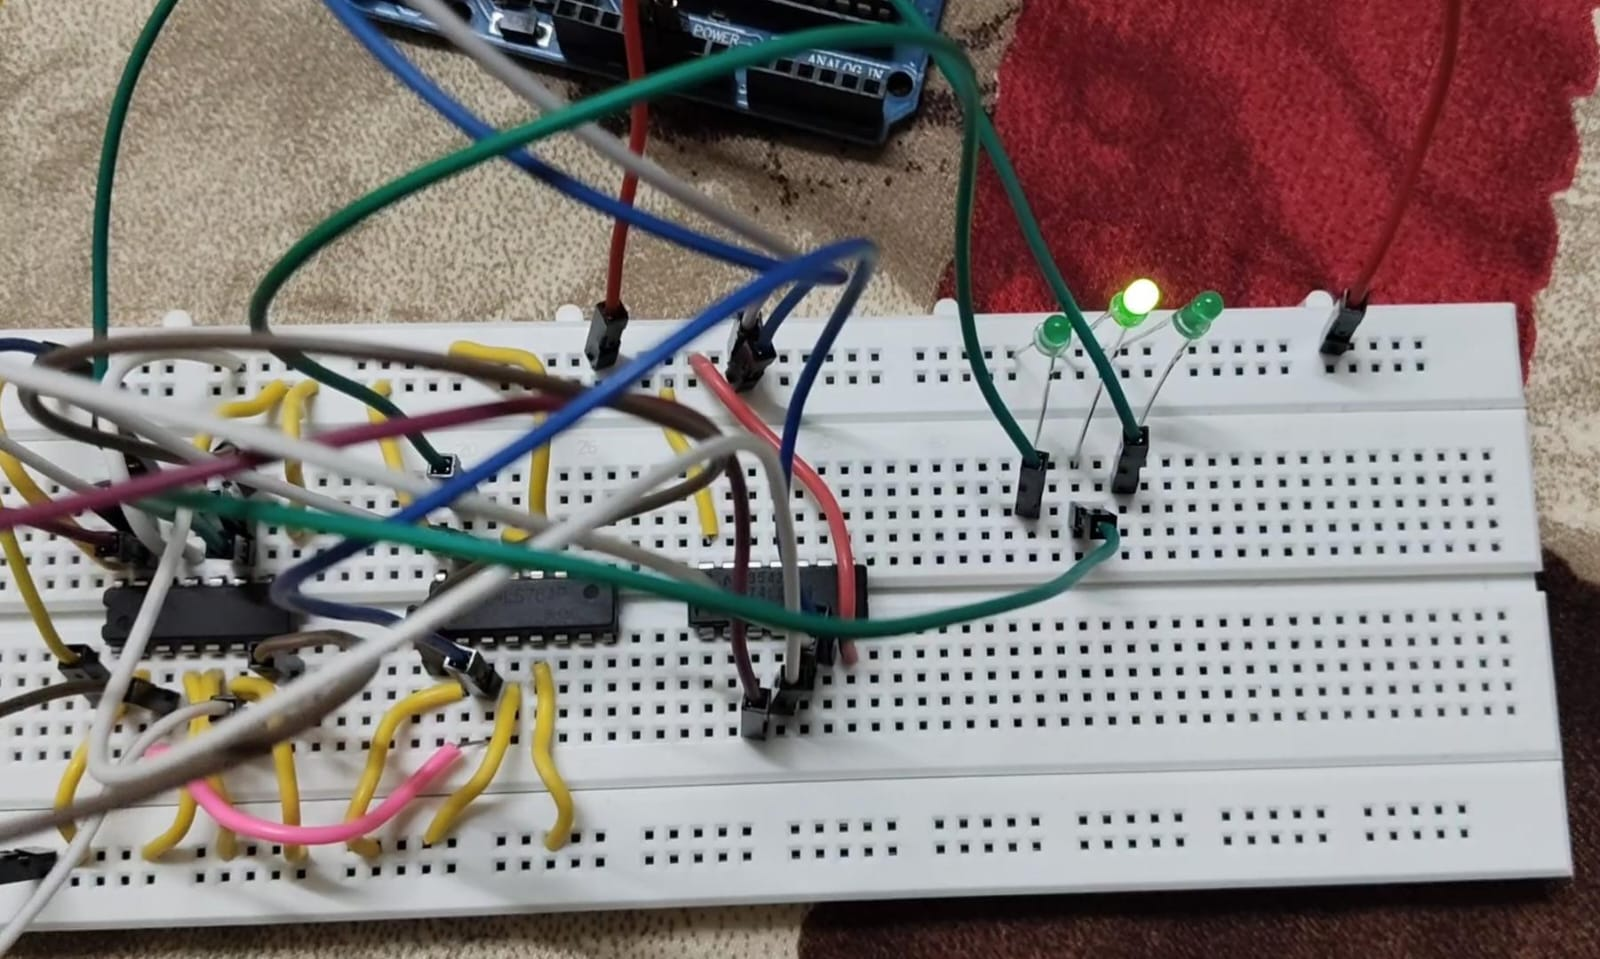
\includegraphics[width=0.6\textwidth]{figs/3.jpeg}
\caption*{0 1 0 = 2}
\end{figure}
\begin{figure}[H]
\centering
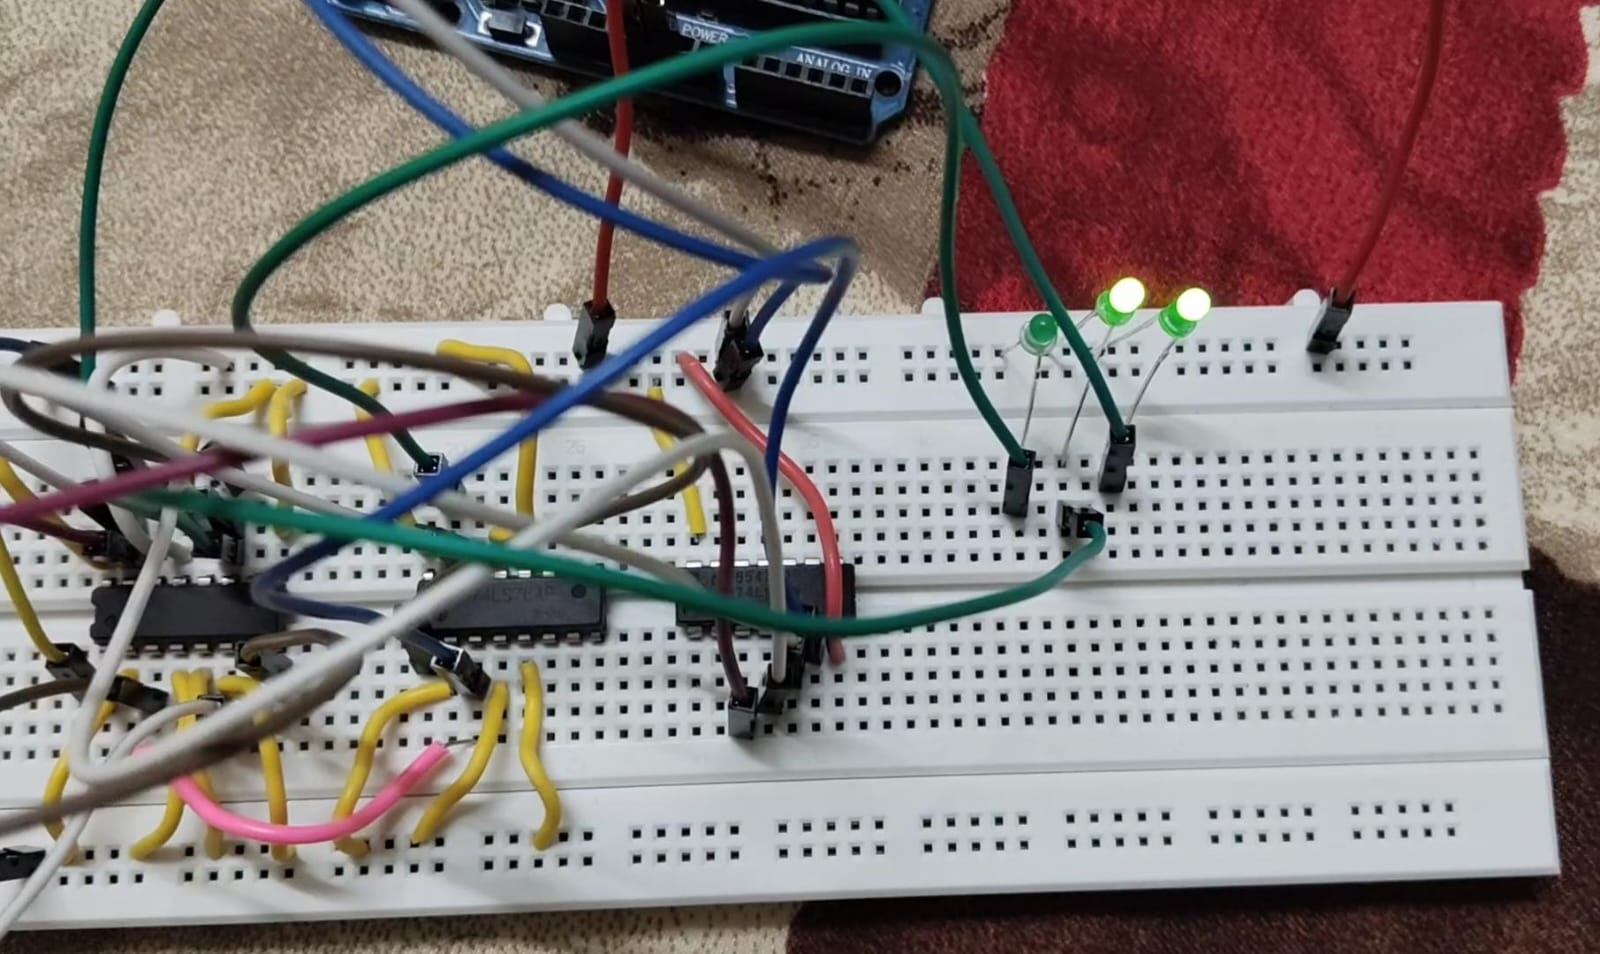
\includegraphics[width=0.6\textwidth]{figs/4.jpeg}
\caption*{0 1 1 = 3}
\end{figure}
\begin{figure}[H]
\centering
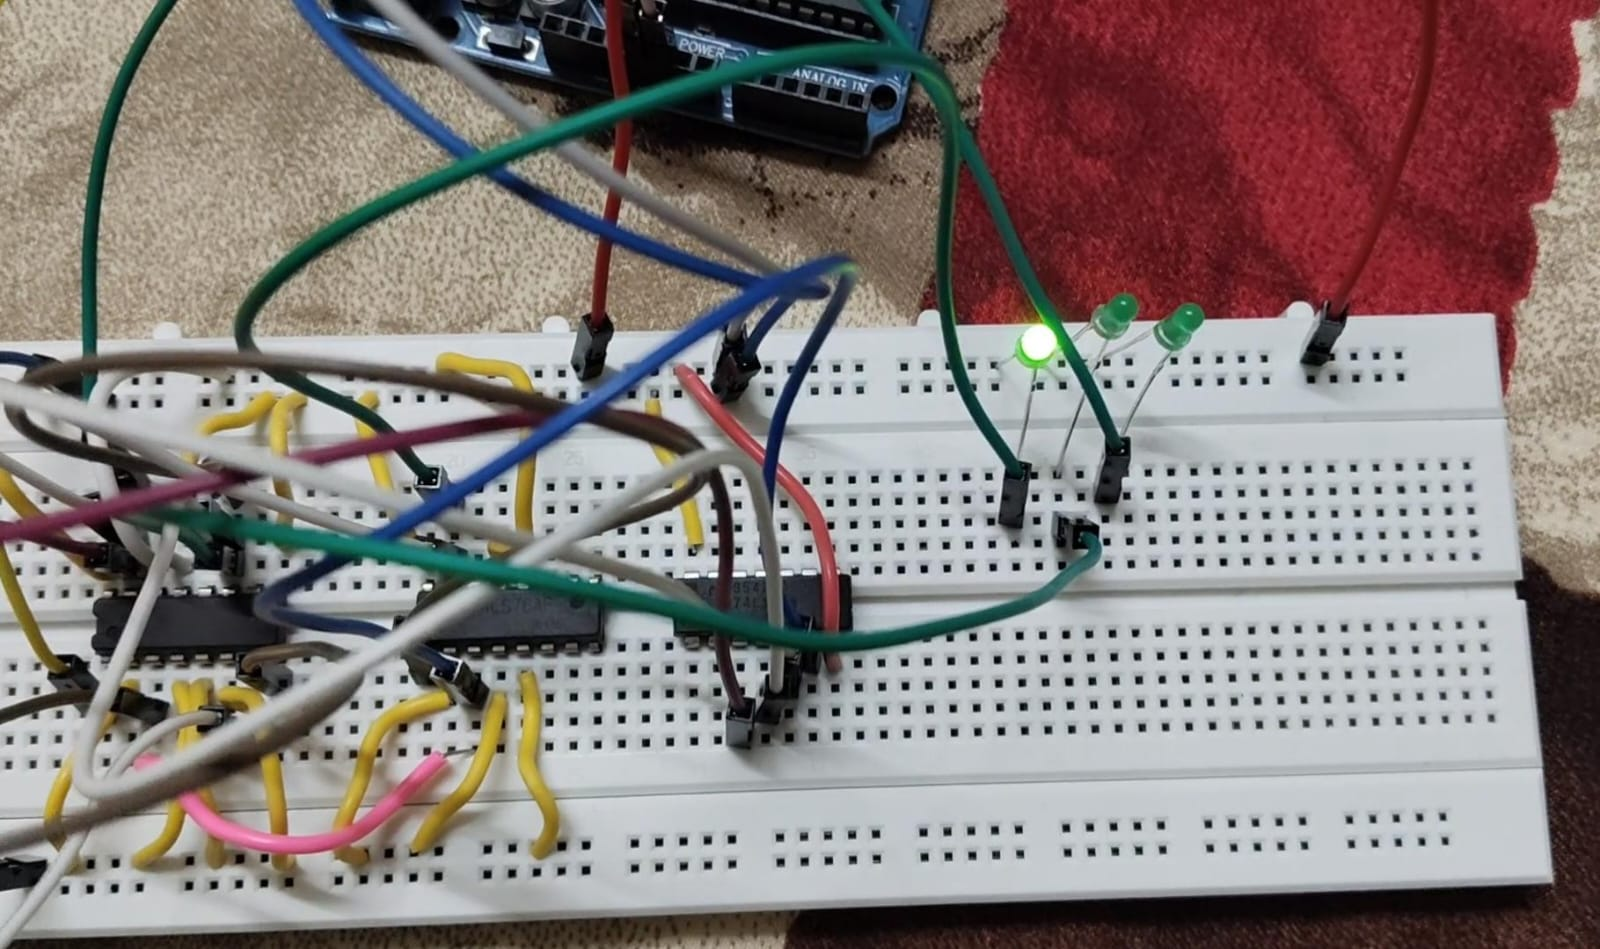
\includegraphics[width=0.6\textwidth]{figs/5.jpeg}
\caption*{1 0 0 = 4}
\end{figure}
\begin{figure}[H]
\centering
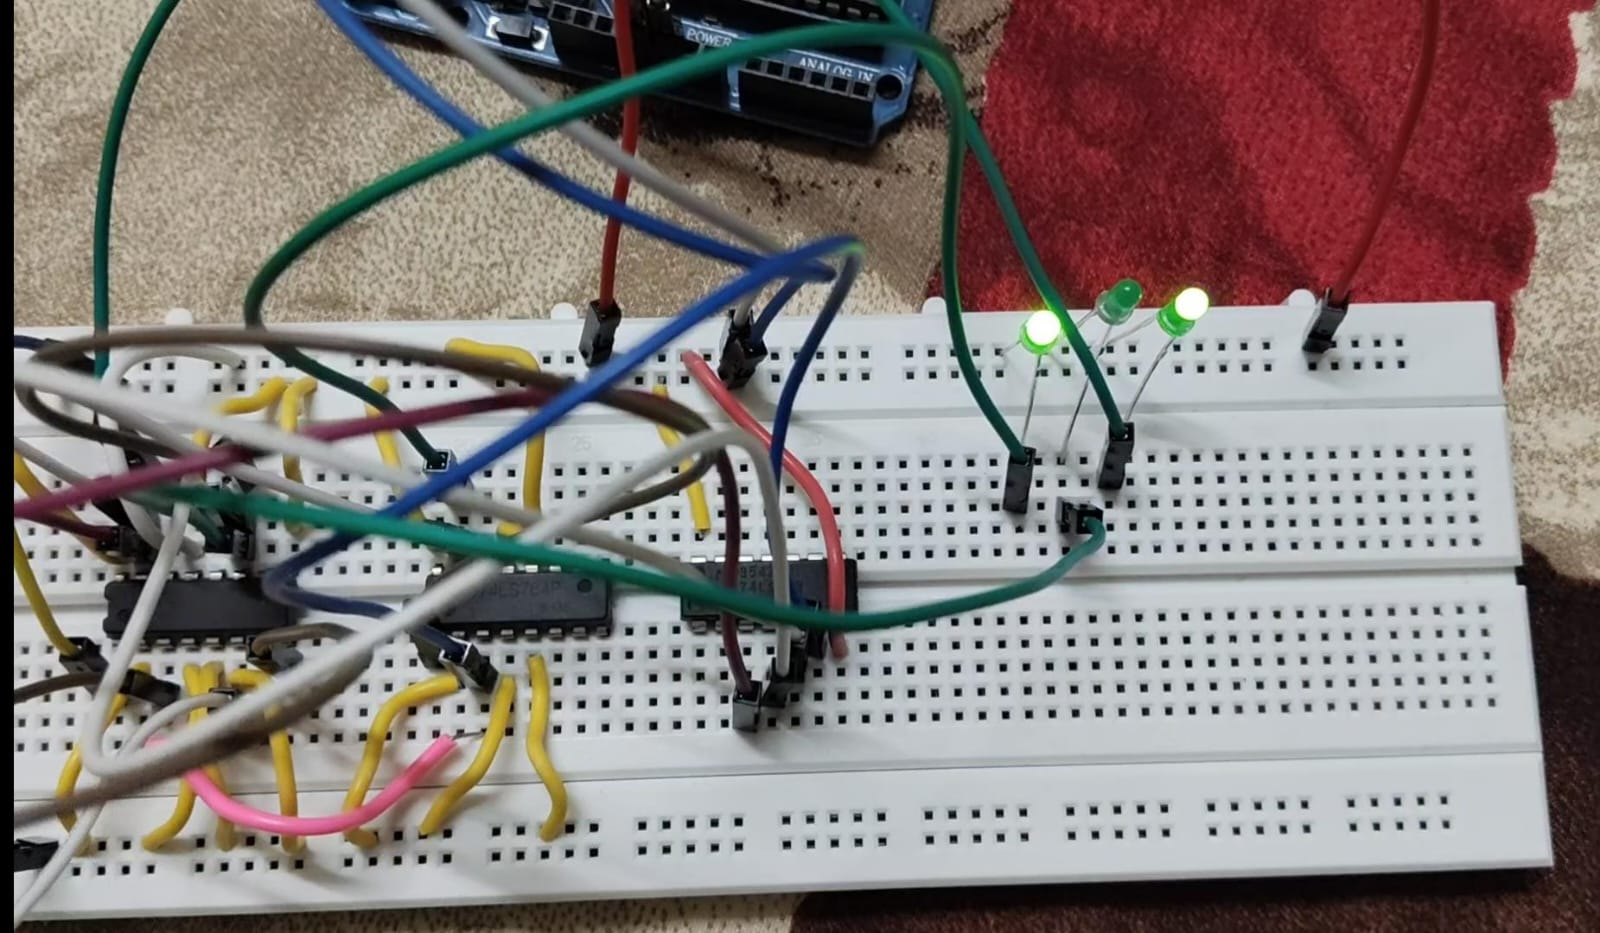
\includegraphics[width=0.6\textwidth]{figs/6.jpeg}
\caption*{1 0 1 = 5}
\end{figure}
\begin{figure}[H]
\centering
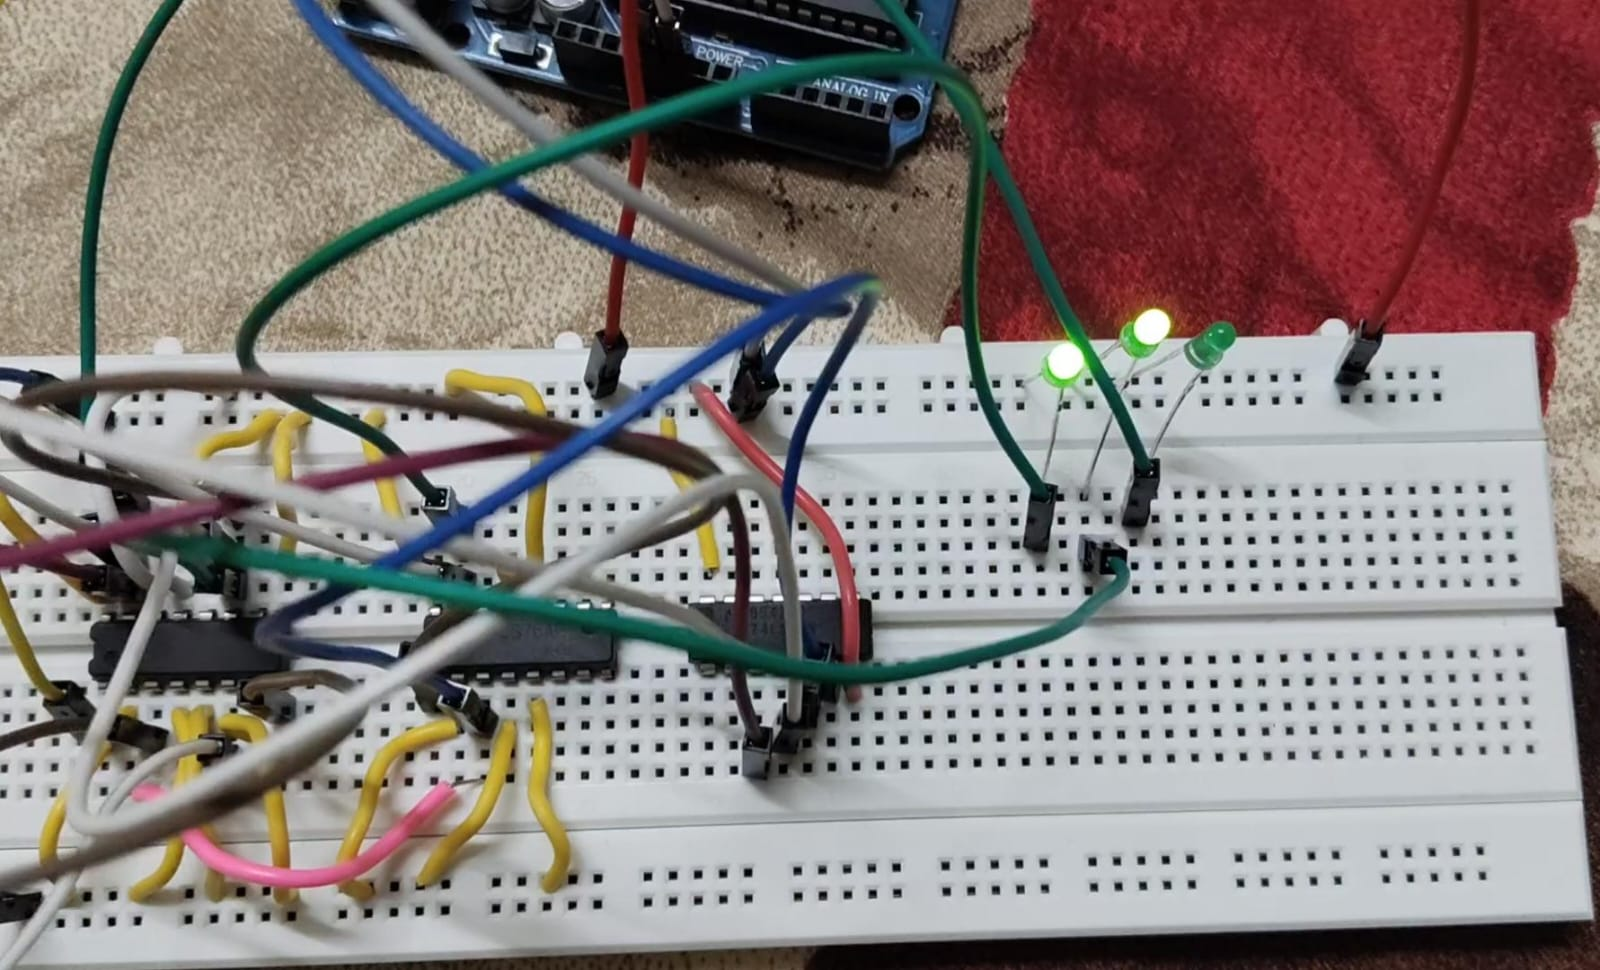
\includegraphics[width=0.6\textwidth]{figs/7.jpeg}
\caption*{1 1 0 = 6}
\end{figure}
\begin{figure}[H]
\centering
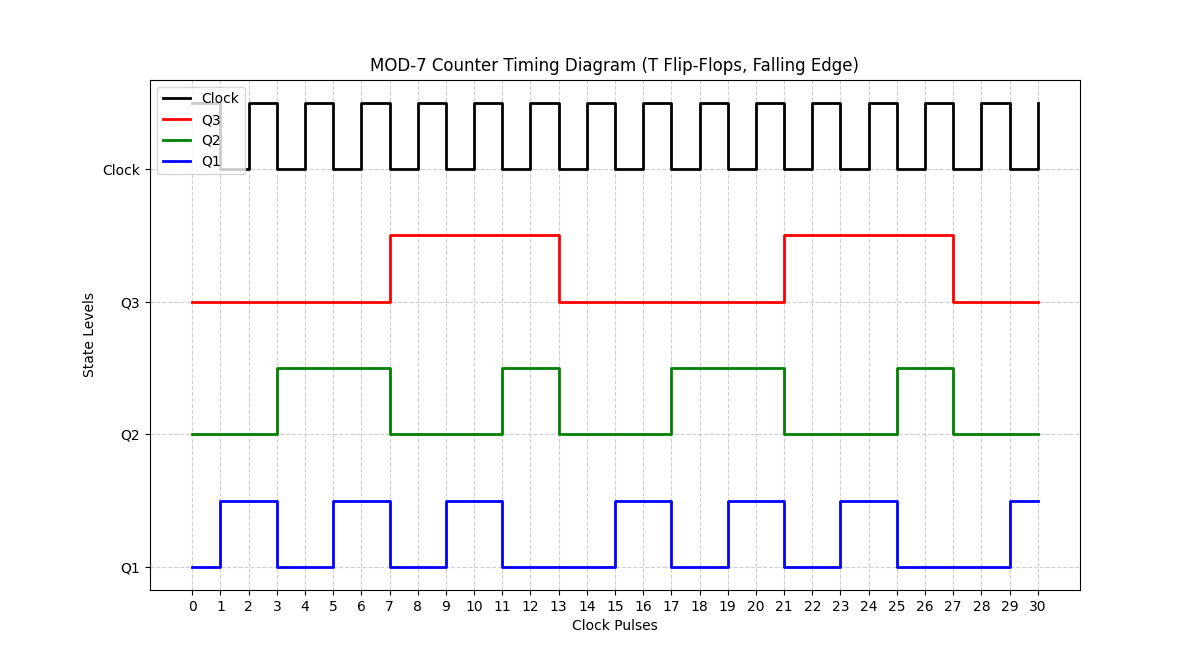
\includegraphics[width=1.1\textwidth]{figs/Plot.png}
\end{figure}
\begin{figure}[H]
\centering
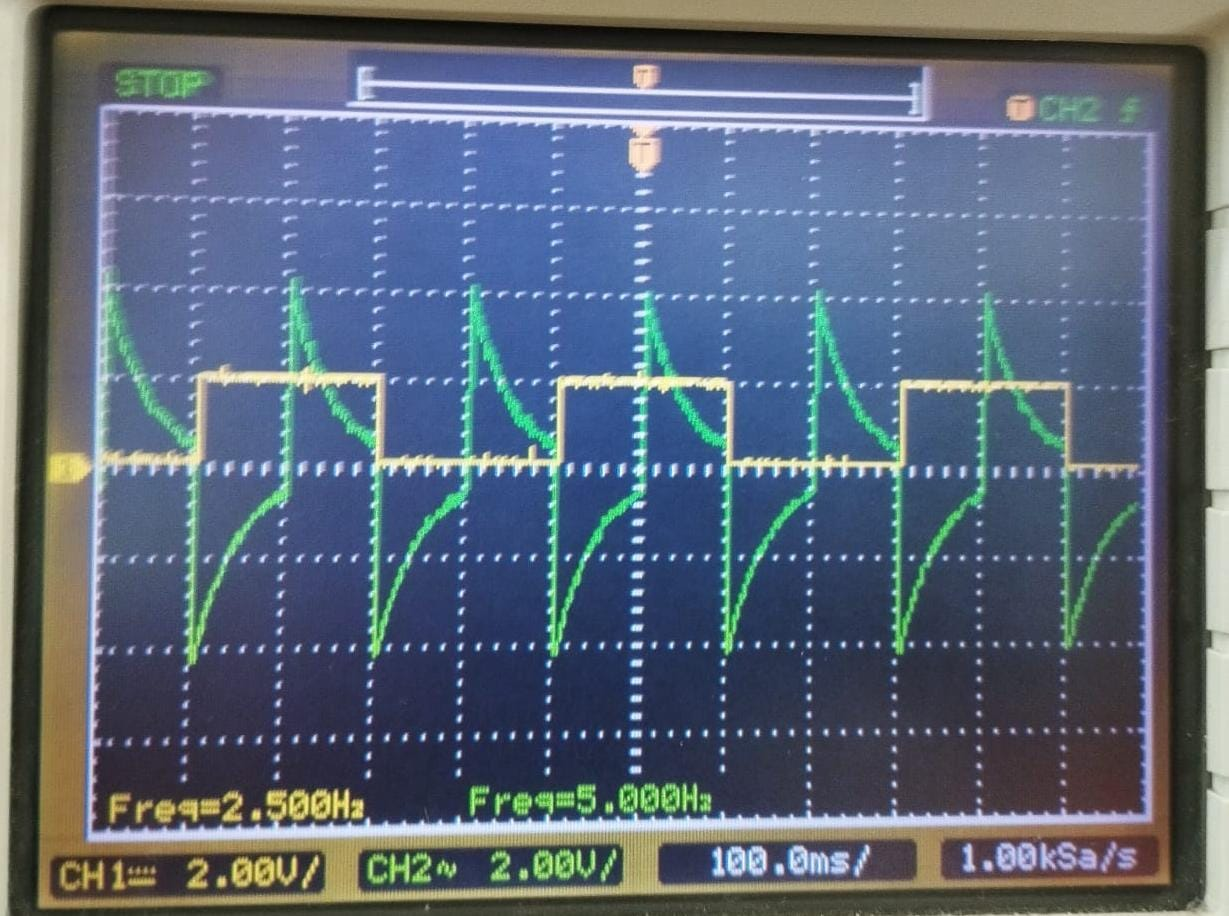
\includegraphics[width=0.6\textwidth]{figs/fig1.jpeg}
\caption{Clock and Q1}
\end{figure}
\begin{figure}[H]
\centering
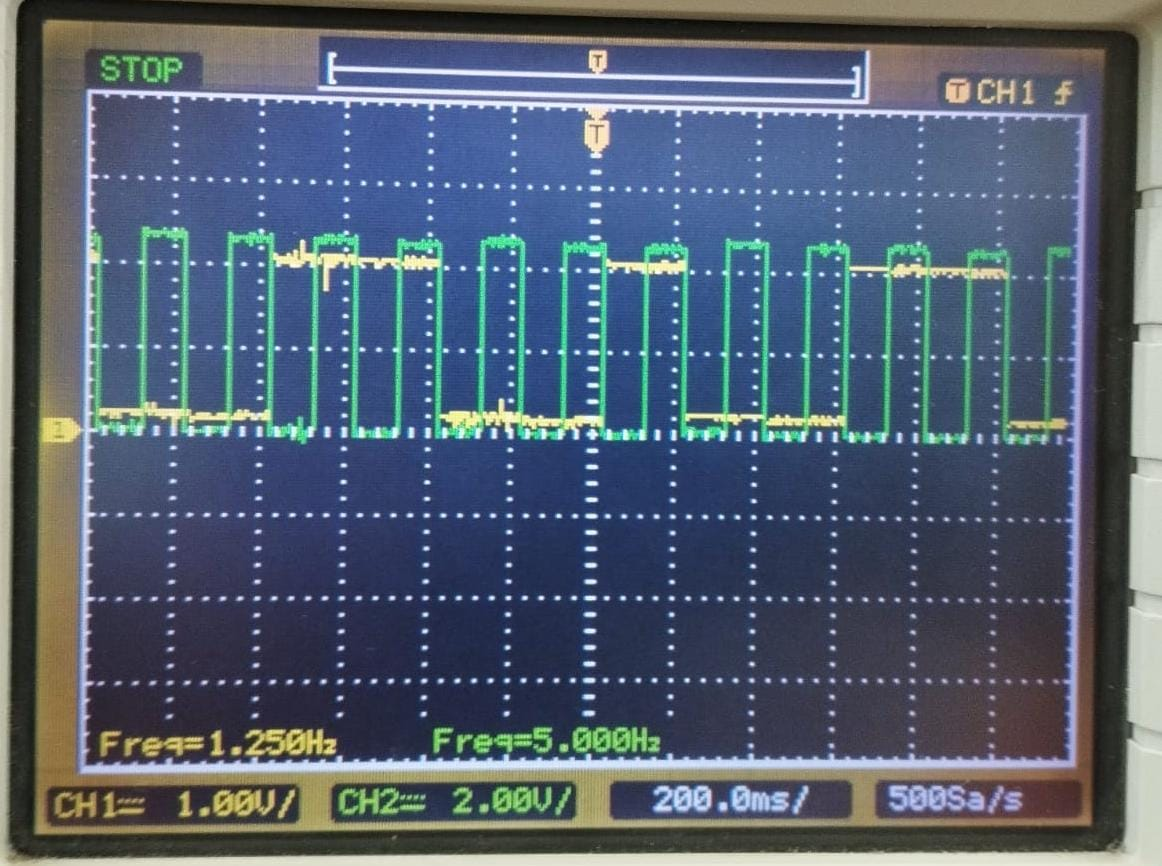
\includegraphics[width=0.6\textwidth]{figs/fig2.jpeg}
\caption{Clock and Q2}
\end{figure}
\begin{figure}[H]
\centering
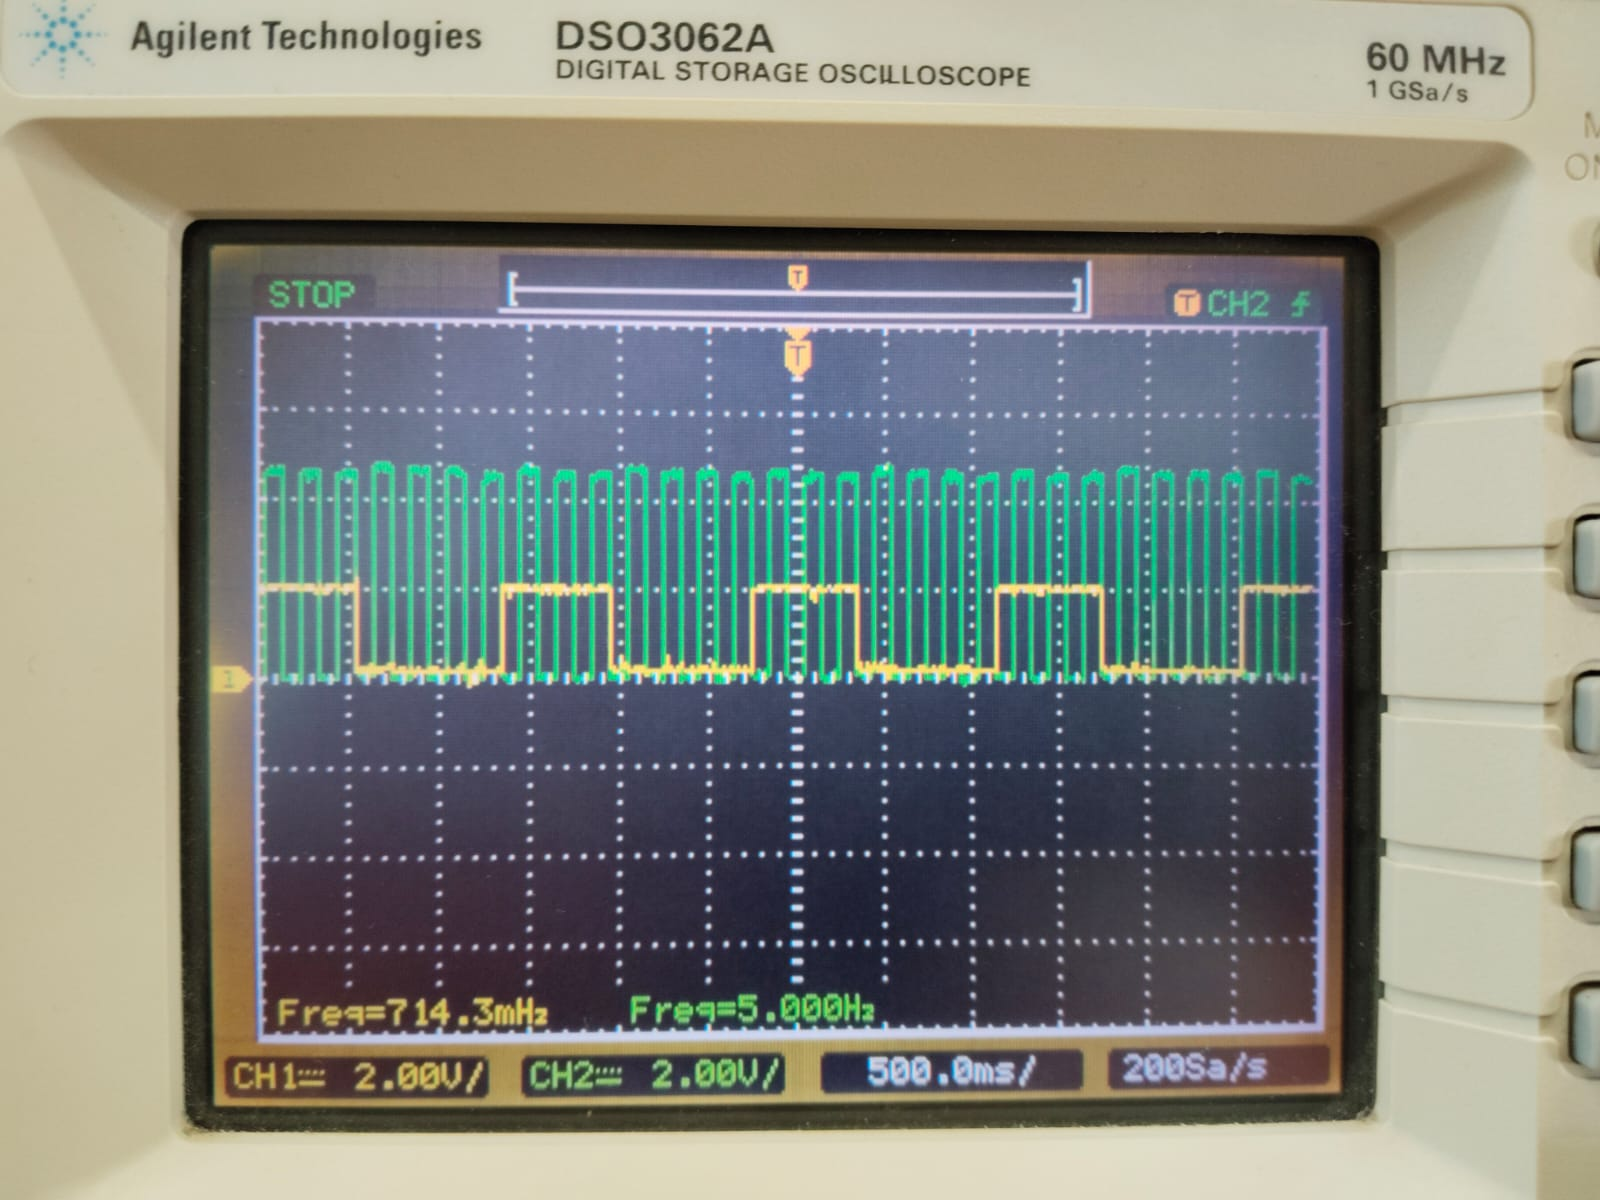
\includegraphics[width=0.6\textwidth]{figs/fig3.jpeg}
\caption{Clock and Q3}
\end{figure}
\section{Conclusion}
The Mod-7 asynchronous counter was successfully designed and tested using JK flip-flops. The circuit counted correctly through seven states and reset as expected. The Arduino provided a stable clock signal, and the output was verified using a CRO.

\end{document}
